\section{Automated Data Collection}
\begin{tcolorbox}[title=One Man's Trash...]
It's been said that the streets of the Web are paved with data that cannot wait to be collected, but you'd be surprised by how much trash there is out there. \\[-0.6cm]
\begin{flushright}
-- Patrick Boily, 2020
\end{flushright}
\end{tcolorbox}
\noindent The way we \textbf{share}, \textbf{collect}, and \textbf{publish} data has changed over the past few years due to the ubiquity of the \textit{World Wide Web}. \textbf{Private businesses}, \textbf{governments}, and \textbf{individual users} are posting and sharing all kinds of data and information. At every moment, new channels generate vast amounts of data.

There was a time in the recent past where both scarcity and inaccessibility of data was a problem for researchers and decision-makers. That is \textbf{emphatically} not the case anymore.
\newl Data abundance carries its own set of problems, however, in the form of 
\begin{itemize}[noitemsep]
\item tangled masses of data, and 
\item traditional data collection methods and classical data analysis techniques not being up to the task anymore (which is not to say that the results they would give would be incorrect; it's rather their lack of efficiency that comes into play).
\end{itemize}
The growth and increasing popularity and power of \textbf{open source software}, such as \text{R} and \text{Python}, for which the source code can be inspected, modified, and enhanced by anyone, makes program-based automated data collection quite appealing. 

One note of warning, however: time marches on and packages become \textbf{obsolete} in the blink of an eye. If the analyst is unable (or unwilling) to \textbf{maintain their extraction/analysis code} and to \textbf{monitor the sites} from which the data is extracted, the choice of software will not make much of a difference. 
\newpage\noindent
So why bother with automated data collection? Common considerations include:
\begin{itemize}[noitemsep]
    \item the sparsity of financial resources;
\item the lack of time or desire to collect data manually;
\item the desire to work with up-to-date, high-quality data-rich sources, and
\item the need to document the analytical process from beginning (data collection) to end (publication).
\end{itemize} 
Manual collection, on the other hand, tends to be cumbersome and prone to error; non-reprodu\-ci\-ble processes are also subject to heightened risks of ``death by boredom'', whereas program-based solutions are typically more reliable, reproducible, time-efficient, and produce datasets of higher quality (this assumes, of course, that coherently presented data exists in the first place).  
\subsection{Automated Data Collection Checklist} That being said, \textbf{web scraping} or \textbf{statistical text processing} is not always recommended. As a start, it is possible that no online and freely available source of data meets the analysis' needs, in which case an approach based on survey sampling is probably indicated. \newl If most of the answers to the following questions are positive, then an automated approach may be the right choice.
\begin{itemize}[noitemsep]
\item Is there a need to repeat the task from time to time (e.g. to update a database)?
\item Is there a need for others to be able to replicate the data collection process?
\item Are online sources of data frequently used?
\item Is the task non-trivial in terms of scope and complexity?
\item If the task can be done manually, are the financial resources required to let others do the work lacking?
\item Is the will to automate the process by means of programming there?
\end{itemize}
The objective is simple: automatic data collection should yield a collection of unstructured or unsorted datasets, at a reasonable cost. 
\subsection{Ethical Considerations} We now turn our attention to a burning question for consultants and analysts alike: is all the freely available data on the Internet ACTUALLY freely available? 
\newl A \textbf{spider} is a program that grazes or crawls the web rapidly, looking for information. It jumps from one page to another, grabbing the entire page content. \textbf{Scraping} is taking specific information from specific websites (which is the goal): how are these different? 
\begin{quote}``Scraping inherently involves \textbf{copying}, and therefore one of the most obvious claims against scrapers is copyright infringement.'' \cite{DC_MRMN}\end{quote}
What can be done to minimize the risk? 
\begin{itemize}[noitemsep]
\item work as transparently as possible;
\item document data sources at all time;
\item give credit to those who originally collected and published the data;
\item if you did not collect the information, you probably need permission to reproduce it, and, more importantly, 
\item don't do anything illegal.
\end{itemize}
A number of  cases have shown that the courts have not yet found their footing in this matter  (see \textit{eBay} vs. \textit{Bidder's Edge}, \textit{Associated Press} vs. \textit{Meltwater}, \textit{Facebook} vs. \textit{Pete Warden}, \textit{United States} vs. \textit{Aaron Swartz}, for instance \cite{DC_M}). There are legal issues that we are not qualified to discuss, but in general, it seems as though larger companies/organisations usually emerge victorious from such battles. \newl Part of the difficulty is that it is not clear which scraping actions are illegal and which are legal. There are rough guidelines: re-publishing content for commercial purposes is considered more problematic than downloading pages for research/analysis, say. A site's  \texttt{robots.txt} (Robots Exclusion Protocol) file tells scrapers what information on the site may be harvested with the publisher's consent -- heed that file (see Figure~\ref{fig:robots} for an example).
\begin{figure}[t]
\centering
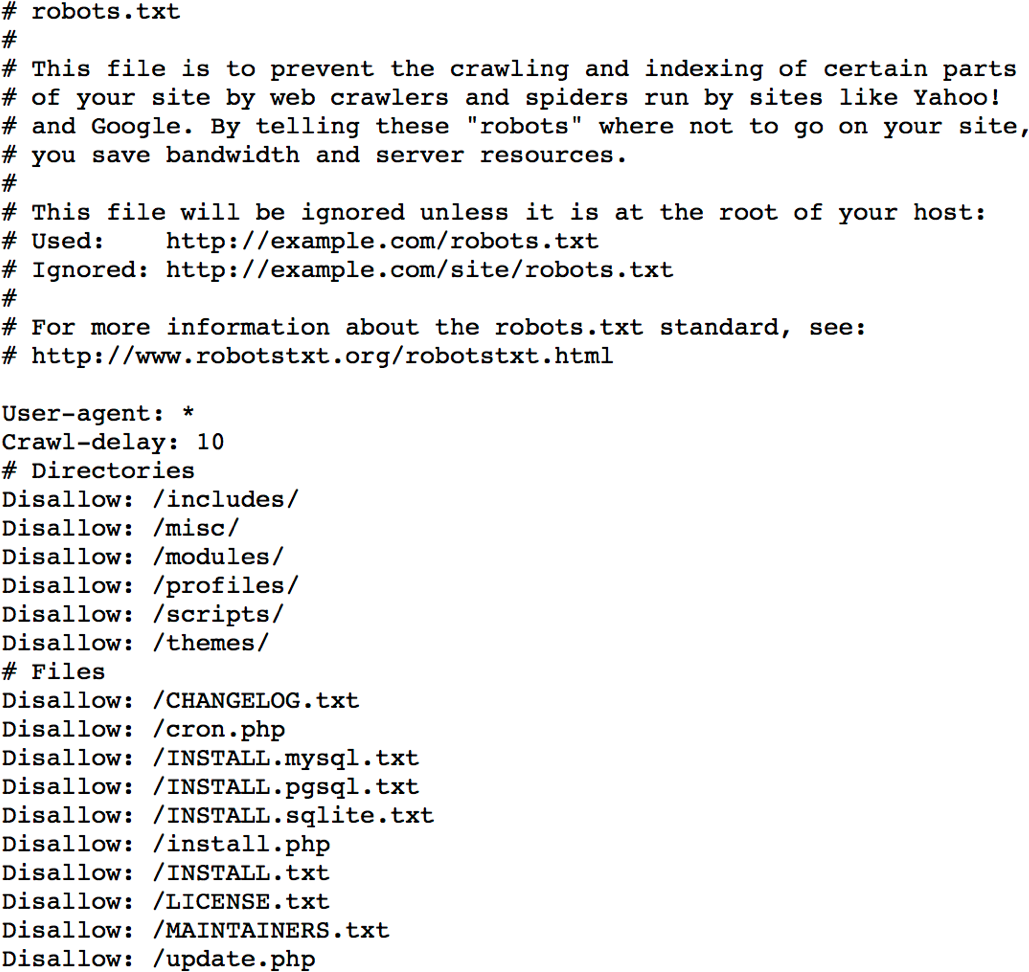
\includegraphics[width=0.50\textwidth]{Images/CQADS_robots.png}
\caption[\small \texttt{robots.txt} file for a random webpage]{\small \texttt{robots.txt} file for \newhref{cqads.carleton.ca}{cqads.carleton.ca}.}\hrule\label{fig:robots}
\end{figure}
\afterpage{\FloatBarrier}
\newl Perhaps more importantly, \textbf{be friendly!} Not everything that can be scraped needs to be scraped. Scraping programs should 1) behave ``nicely''; 2) provide useful data, and 3) be efficient, in that order. When in doubt, contact the data provider to see if they will grant access to the databases or files. 
\newpage\noindent Finally, note the importance of following the \textbf{Scraping Do's and Don't's}:
\begin{enumerate}[noitemsep]
    \item \textbf{stay identifiable};
    \item \textbf{reduce traffic} -- accept compressed files, check that a file has been changed before accessing it again, retrieve only parts of a file;
    \item \textbf{do not bother server with multiple requests} --  many requests per second can bring smaller server downs, webmasters may block you if your scraper is too greedy (a few requests per second is fine), and
    \item \textbf{write efficient and polite scrapers} -- there is no reason to scrape pages daily or to repeat the same task over and over, select specific resources and leave the rest untouched. 
\end{enumerate}
\subsection{Web Data Quality} Data quality issues are inescapable. It is not rare for clients to have spent thousands of dollars on data collection (automatic or manual) and to respond to the news that the data is flawed or otherwise unusable with: ``well, it's the best data we have, so find a way to use it.''\par These issues can be side-stepped to some extent if consultants get involved in the project during or prior to the data collection stage, asking questions such as:
\begin{itemize}[noitemsep]
    \item what type of data is best-suited to answer the client's question(s)?
    \item is the available data of sufficiently high quality to answer the client's question(s)?
    \item is the available information systematically flawed?
\end{itemize}
Web data can be \textbf{first-hand} information (a tweet or a news article), or \textbf{second-hand} (copied from an offline source or scraped from some online location, which may make it difficult to retrace). \textbf{Cross-referencing} is a standard practice when dealing with secondary data.  \newl Data quality also depends on its \textbf{use(s)} and \textbf{purpose(s)}. For example,
a sample of tweets collected on a random day could be used to analyse the use of a hashtags or the gender-specific use of words, but that dataset might not prove as useful if it had been collected on the day of the 2018 U.S. Presidential Election to predict the election outcomes (due to \textbf{collection bias}).
\newl An example might help to illustrate some the pitfalls and challenges. Let's say that a client is interested in finding out what people think of a new potato peeler using a standard telephone survey. 
Such an approach has a number of pitfalls:
\begin{itemize}[noitemsep]
\item\textbf{unrepresentative sample} -- the selected sample might not represent the intended population;
\item\textbf{systematic non-response} -- people who don't like phone surveys might be less (or more) likely to dislike the new potato peeler;  
\item\textbf{coverage error} -- people without a landline can't be reached, say, and 
\item\textbf{measurement error} -- are the survey questions providing suitable info for the problem at hand?
\end{itemize}
Traditional solutions to these problems require the use of survey sampling (more on this later), questionnaire design (see previous section), omnibus surveys, reward systems, audits, etc. These solutions can be \textbf{costly}, \textbf{time-consuming}, and \textbf{ineffective}. \newl \textbf{Proxies} -- indicators that are strongly related to the product's popularity without measuring it directly, could be useful. If \textbf{popularity} is defined as large groups of people preferring a potato peeler over another one, then sales statistics on a commercial website may provide a proxy for popularity. 
\newl Rankings on \texttt{Amazon.ca} (or a similar website) could, in fact, paint a more comprehensive portrait of the potato peeler market than would a traditional survey. It would suffice, then, to build a scraper that is compatible with Amazon's \textbf{application program interface} (API) to gather the appropriate data.\newl Of course, there are potential issues with this approach as well: 
\begin{itemize}[noitemsep]
\item \textbf{representativeness} of the \textbf{listed products} -- are all potato peelers listed? If not, is it because that website doesn't sell them? Is there some other reason?
\item \textbf{representativeness} of the \textbf{customers} -- are there specific groups buying/not-buying online products? Are there specific groups buying from specific sites? Are there specific groups leaving/not-leaving reviews? 
\item \textbf{truthfulness} of customers and \textbf{reliability} of reviews -- how can we distinguish between paid (fake) reviews and real reviews?
\end{itemize}
Web scraping is usually well-suited for collecting data on products (such as the aforementioned potato-peeler), but there are numerous questions for which it is substantially more difficult to imagine where data could be found online: what data could you collect online to measure the popularity of a government policy, say? 
\subsection{Web Technologies 101}
Online data can be found in \textbf{text}, \textbf{tables}, \textbf{lists}, \textbf{links}, and other structures, but the way data is presented in browsers is not necessarily how it is stored in HTML/XML. Furthermore, when web pages are \textbf{dynamic}, there is a ``cost'' associated with automated collection. Consequently, a basic knowledge of the web and web-related techs and documents is crucial. Information is readily available online (see references) and in  \cite{DC_M,DC_MRMN}.\newpage\noindent There are three areas of importance for data collection on the web:
\begin{itemize}[noitemsep]
\item technologies for \textbf{content dissemination} (HTTP, HTML/XML, JSON, plain text, etc.);
\item technologies for \textbf{information extraction} (R, Python, XPath, JSON parsers, Beautiful Soup, Selenium, regexps, etc.), and 
\item technologies for \textbf{data storage} (R, Python, SQL, binary formats, plain text formats, etc.).
\end{itemize}
Webpage content itself comes into three main categories: Hypertext Markup Language (HTML; used for web content and code), Cascading Style Sheets (CSS; used for webpage style), and 
JavaScript (js; used for interactivity with the webpage). HTML is, in some sense, the most fundamental; understanding the tree structure of HTML documents, for instance, will go a long way towards helping consultants get full use of the \textbf{scraping toolbox}. 
\subsection{Scraping Toolbox} From experience, we know that a number of tools can facilitate the automated data extraction process, including: 
\textit{Developer Tools}, \textit{XPath}, \textit{Beautiful Soup}, \textit{Selenium}, and \textit{regular expressions}. 
\newl\textbf{Developer Tools} show the correspondence between the HTML code for a page and the rendered version seen in the browser (see Figure~\ref{fig:erb} for an example). Unlike ``View Source'', Developer Tools show the \textit{dynamic} version of the HTML content (i.e. the HTML is shown with any changes made by JavaScript since the page was first received). Inspecting a page's various elements and discovering where they reside in the HTML file is \textbf{crucial} to efficient web scraping: 
\begin{figure*}[t]
\centering
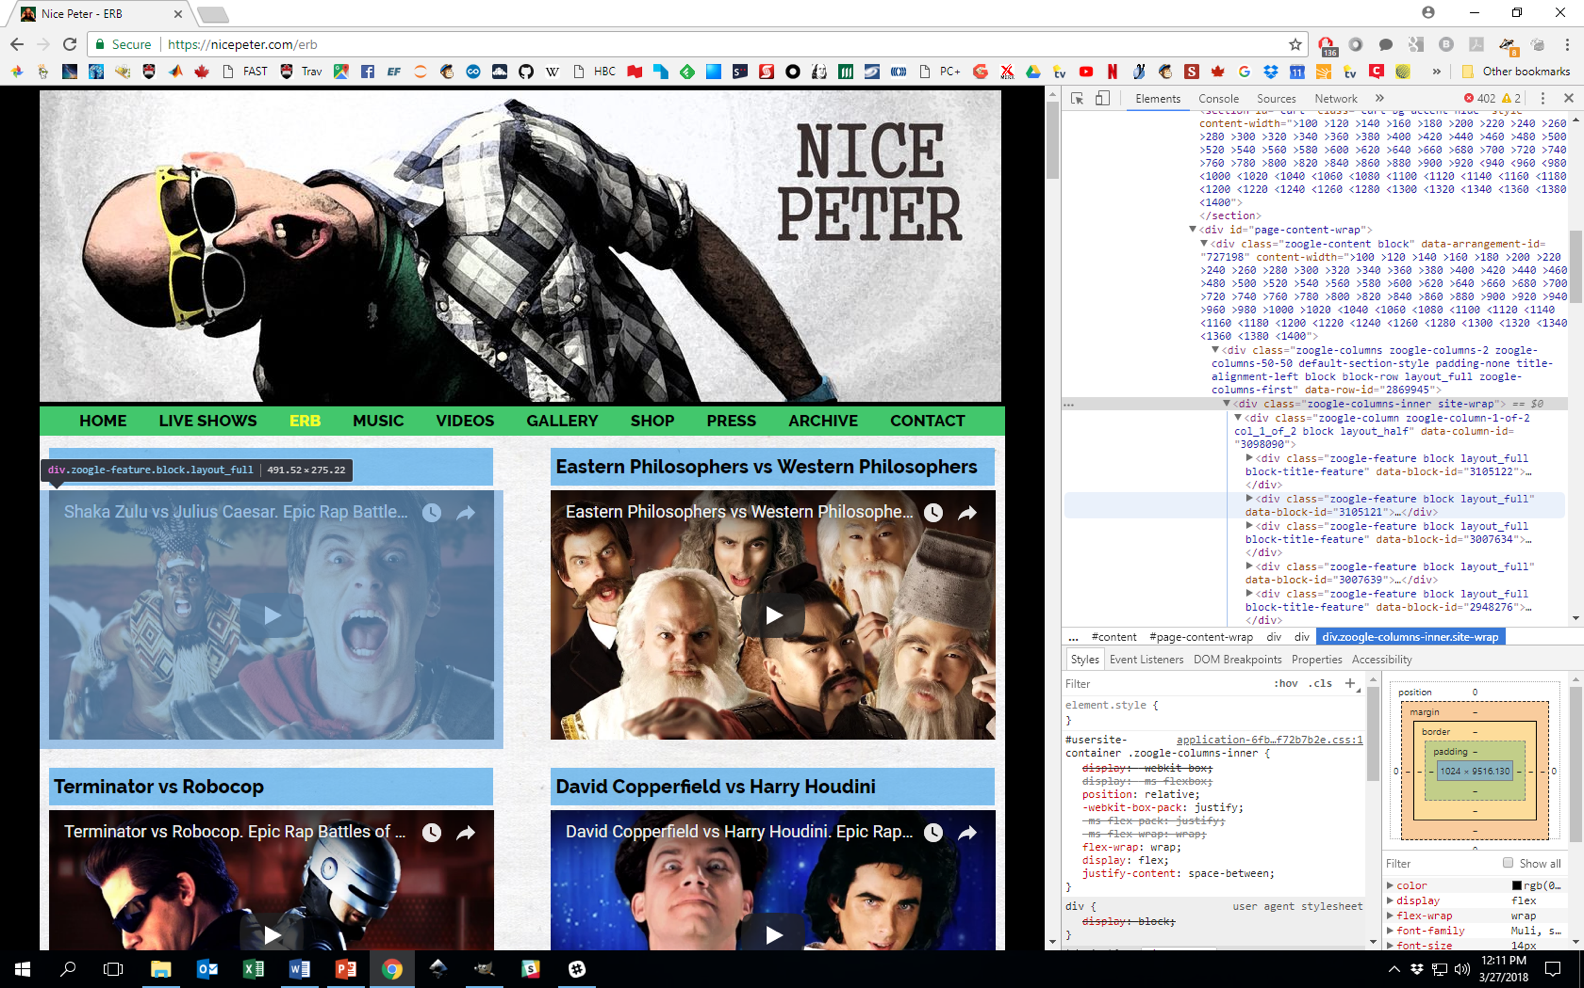
\includegraphics[width=\textwidth]{Images/erb.png}
\caption[\small Inspecting a webpage elements using Chrome's \textit{Developer Tools}]{\small Inspecting \newhref{https://nicepeter.com/erb}{https://nicepeter.com/erb}'s elements using Chrome's \textit{Developer Tools}.} \hrule\label{fig:erb}
\end{figure*}
\begin{itemize}[noitemsep]
\item \textbf{Firefox} -- right click page $\to$ Inspect Element
\item \textbf{Safari} -- Safari $\to$ Preferences $\to$ Advanced $\to$ Show Develop Menu in Menu Bar, then  
Develop $\to$ Show Web Inspector
\item \textbf{Chrome} --  right click page $\to$ Inspect
\end{itemize}
\textbf{XPath} is a query (domain-specific) language which is 
used to select specific pieces of information from marked-up documents such as HTML, XML, or variants such as SVG, RSS. Before this can be done, the information stored in a marked-up document needs to be converted (or \textbf{parsed}) into a format suitable for processing and statistical analysis; this is implemented in the R package XML, for instance. The process is simple; it involves 
\begin{enumerate}[noitemsep]
\item specifying the data of interest;
\item locating it in a specific document, and
\item tailoring a query to the document to extract the desired info.
\end{enumerate}
XPath queries require both a \textbf{path} and a \textbf{document} to search; paths consist of hierarchical addressing mechanism (succession of nodes, separated by forward slashes (``/''), while a query takes the form \small\texttt{xpathSApply(doc,path)}\normalsize :\\
\footnotesize\texttt{xpathSApply(parsed\_doc,``/html/body/div/p/i'')}\normalsize, for instance, would find all \texttt{<i>} tags found under a \texttt{<p>} tag, itself found under a \texttt{<div>} tag in the \texttt{body} of the \texttt{html} file of \texttt{parsed\_doc}. Consult \cite{DC_MRMN} for a substantially heftier introduction. 
\newl\textbf{Regular Expressions} can be used to achieve the main web scraping objective, which is to extract  relevant information from reams of data. Among this mostly unstructured data lurk \textbf{systematic elements}, which can be used to help the automation process, especially if quantitative methods are eventually going to be applied to the scraped data. Systematic structures include numbers, names (countries, etc.), addresses (mailing, e-mailing, URLs, etc.), specific character strings, etc. Regular expressions (regexps) are abstract sequences of strings that match concrete recurring patterns in text; they allow for the systematic extraction of the information components from plain text, HTML, and XML. Some examples that illustrate the main concepts are shown in the accompanying \textit{Jupyter Notebooks}. %showcased in Section~\ref{sec:docs}. 
\newl\textbf{Beautiful Soup} is a Python library that helps extract data out of HTML and XML files. It parses HTML files, even if they're broken. Beautiful Soup does not simply convert bad HTML to good X/HTML; it allows a user to fully inspect the (proper) HTML structure it produces, in a programmatical fashion. When Beautiful Soup has finished its work on an HTML file, the resulting \textit{soup} is an API for \textbf{traversing}, \textbf{searching}, and \textbf{reading} the document's elements. In essence, it provides \textbf{idiomatic} ways of navigating, searching, and modifying the parse tree of the HTML file, which can save a fair amount of time.
\par For instance, \texttt{soup.find\_all('a')} would find and output all \texttt{<a ...> ... </a>} tag pairs (with attributes and content) in the \texttt{soup}, whereas \begin{quote}\texttt{for link in soup.find\_all('a'):}\newline \texttt{\ \ \ print(link.get('href')}
\end{quote} would output the URLs found in the same tag pairs. The Beautiful Soup documentation is quite explicit and provides numerous examples \cite{DC_BS}. 
\newl\textbf{Selenium} is a Python tool used to automate web browser interactions.  It is used primarily for testing purposes, but it has data extraction uses as well. Mainly, it allows the user to open a browser and to act as a human being would:
\begin{itemize}[noitemsep]
    \item clicking buttons;
\item entering information in forms;
\item searching for specific information on a page, etc.
\end{itemize}
Selenium requires a driver to interface with the chosen browser. Firefox, for example, uses \texttt{geckodriver}. Other supported browsers have their own drivers (see \cite{DC_S_C,DC_S_E,DC_S_F,DC_S_S}).

\noindent Selenium automatically controls a complete browser, including rendering the web documents and running JavaScript. This is useful for pages with a lot of dynamic content that isn't in the base HTML. Selenium can program actions like ``click on this button'', or ``type this text'', to provide access to the dynamic HTML of the current state of the page, not unlike what happens in  \textit{Developer Tools} (but now the process can be fully automated). More information can be found in \cite{DC_S,DC_S2}.
\newl 
Let us end this section by providing a short summary of the \textbf{automated data collection decision process} \cite{DC_MRMN,DC_M}, as seen by  quantitative consultants. 
\begin{enumerate}
    \item \textbf{Know exactly what kind of information the client needs}, either \textbf{specific} (e.g. GDP of all OECD countries for last 10 years, sales of top 10 tea brands in 2017, etc.) or \textbf{vague} (people's opinion on tea brand $X$, etc.)
\item \textbf{Find out if there are any web data sources that could provide direct or indirect information on the client's problem.} That is easier to achieve for specific facts (a tea store's webpage will provide information about teas that are currently in demand) than it is for vague facts. Tweets and social media platforms may contain opinion trends; commercial platforms can provide information on product satisfaction.
\item \textbf{Develop a theory of the data generation process when looking into potential data sources.} When was the data generated? When was it uploaded to the Web? Who uploaded the data? Are there any potential areas that are not covered, consistent, or accurate? How often is the data updated?
\item \textbf{Balance the advantages and disadvantages of potential data sources.} Validate the quality of data used -- are there other independent sources that provide similar information against which to crosscheck? Can original source of secondary data be identified?
\item \textbf{Make a data collection decision}. Choose the data sources that seem most suitable, and document reasons for this decision. Collect data from several sources to validate the final choice. 
\end{enumerate}
%\afterpage{\FloatBarrier}